%!TEX program = xelatex
\documentclass[12pt]{article}
\usepackage[utf8]{inputenc}
\usepackage{amsmath,amssymb}
\usepackage{amsthm}
%\usepackage{booktabs}
\usepackage{lmodern,textcomp}
\usepackage{graphicx}
\newcommand{\HRule}{\rule{\linewidth}{0.5mm}}
\usepackage{float}
\usepackage{physics}

\usepackage{url}
\bibliographystyle{plain}


%\usepackage{listings}

\usepackage{parskip}
\setlength{\parindent}{1em}
\linespread{1.25}

\newcommand\diff{\,\mathrm{d}}
\renewcommand{\footnoterule}{\rule{\linewidth}{0pt}}
\renewcommand{\thefootnote}{\fnsymbol{footnote}}

\begin{document}
\title{Case study of Scalable Quantum Simulation of Molecular Energies}
\author{Shuhao Yang, James Mills, Shanice St John}
\date{\today}
\maketitle
\section{Introduction}
“Nature isn't classical, dammit, and if you want to make a simulation of nature, you'd better make it quantum mechanical, and by golly it's a wonderful
 problem, because it doesn't look so easy.” Richard Feynman’s words are as true today as when he spoke them almost forty years ago.

Simulation of physical systems is one of the most crucial practical applications of computation by far.  For example, buildings are engineered in a safe
and cost efficient way though the application of finite element analysis and modeling. The field of aeronautics relies heavily on computational fluid
dynamics simulations. And even nuclear weapons systems are tested by exhaustive computational modeling.

However, even in light of it's phenomenally far-reaching success in almost all areas of modern science and engineering, classical computation still
has its limitations. When it comes to simulating microscopic systems, classical techniques require significant computational overhead which scales to
unreasonable proportions with increasing system size. In quantum computational chemistry simulations, each subatomic orbital and their interactions
needs to be considered to achieve an accurate and realistic simulation of the microscopic system. Since the state of one orbital can be affected by
all of the others, an exponential number of states in the basis of molecular orbitals needs to be accounted for. Problems of this type are classified
to be ‘many-body’ problems. No matter how far apart two orbitals are, their quantum states cannot be described independently, the repeated interactions between particles create
quantum correlations, this phenomenon is known as entanglement.

A radically different computing paradigm is then employed to combat this problem, that is quantum computation. It harnesses the principles of quantum
mechanics, hence solves these classically intractable problems of simulation more accurately, faster, with a more fine-grained simulation.

The amount of information needed to describe interactions in a quantum system would quickly fill up the memory of a classical computer, instead,
a quantum computer can do tasks of this nature efficiently through the use of quantum bits, or qubits, for information storage and computation
\cite{trabesinger2012quantum}. Since the classical storage unit ‘bit’ is binary system based on strings of 0s and 1s, but a quantum computer would
encode them into two distinguishable quantum states, and one qubit can represent multiple states at once in the form of the quantum phenomenon of
‘superposition’. Similarly, if we perform a search algorithm on a classical string, the enumerate steps would be the number of bits within this
string. Comparably, our processing step will reduce a lot more as we only need to compute once in a quantum processor.

\section{History}
Molecules are composed of collections of atoms, and the units that make up an atom are electrons and the atomic nucleus. When we consider the
 atomic energy then we must take into account both electron-nuclei and electron-electron interactions. The molecular energy consists of interactions
 between multiple atoms, and interactions between electrons from different nuclei. Molecular energy can be pictured as a large
 package that contains many small balls, and the sum of the energy of their collisions is the sum of interactions between atoms. Obviously, it
 demands massive computation to find out the package energy as it contains a huge amount of particles. Therefore, some approximations need to be
  made to simply our model, which necessitates the introduction of molecular mechanics.

Molecular mechanics models molecular systems using force fields in classical mechanics. Three approximations were made to reduce the computational
 complexity. Each atom is simulated as one particle; each particle has their designated attributes including radius, Polaris ability and net charge;
 and interactions are treated as springs with an equilibrium distance same as bond length. Essentially this theory simulates every element of the
 molecular system as if it were fixed particles connected by strings, which hugely reduces the computational complexity.

The renormalisation group is a theory which also enables a reduction in the computational power needed for accurate simulations. A simple scenario
is to calculate the resistance force of an iron ball in a glass of water. We can simply simulate every water molecule in the glass by using the
 real size of a single water molecule as one parameter - the sizes of the molecules can easily be another 1000 parameters as they can be
 irregular and difficult to describe. Forces from multiple directions of the iron ball could be another 1000 parameters. Inputting all parameters,
  modelling an iron ball and simulating $10^{26}$ water molecules and their interactions can give the resistance force. Let’s say we have a
  supercomputer that allows for a tremendous amount of data processing and the result that this simulation gives coincides with the experimental data
  to within an extremely high degree of accuracy.

But what if we want to reduce the computational complexity? One solution is to reduce the number of water molecules simulated, which is feasible given
 the relative much larger size of the iron ball. To make up for the loss in number of molecules, the rest if the parameters can be adapted. Whereby we
can manipulate the parameters and the simulation gives slightly different solutions, but the overall trend is still the same as before. The computation
 complexity can still be compressed. We can repeat the process of reducing the number of molecules and adjusting the parameters and still generate
  acceptable solutions. This process is known as renormalisation group, and the results that this model generates are called low energy effective
  theory, in which the system size is reduced but the results are still accurate.

We now return to the theory of molecular mechanics, it is not exactly accurate since it is restricted by parameters of equations, i.e. different
force fields for different atoms. A similar and perhaps more comprehensible explanation can be made from the theory of renormalisation group.
While decreasing the parameters of calculation and reducing computation time, the accuracy of the result is decreasing as well. Molecular mechanics
 does the same for force fields and interactions inside the atom.

Overall, the work on simulating molecular energies with classical methods is a trade off between precision and cost. Quantum simulation is able
to encapsulate all the relevant information of the system, and can simulate efficiently and without approximations.

\section{Non-technical background}

In any quantum computing processes, the building blocks of the process are qubits. A qubit, or quantum bit, is the quantum analogue of the classical
 bit (strings of zeros and ones). So the qubit represents a quantum superposition or combination of a predetermined ‘0’ and a ‘1’ state. The quantum
  algorithms were run on superconducting qubits, these are a physical realisation of quantum bits based upon what are known as superconducting
  interference devices (SQUIDs), and attempt to find properties of the wavefunction of the molecule (in this case molecular Hydrogen).

The wavefunction of a quantum system is a mathematical construct describing the state, it provides probabilities for results of particular measurements
 made on the state. In quantum chemistry the electronic structure of a molecule is described by the movement of the electrons of a collection of fixed
  atomic nuclei. And so a comprehensive description of the electronic structure encompasses the wavefunctions of all of these electrons, along with
  their respective energies. The idea that the motions of the electrons and nuclei may be considered separately is known as the Born-Oppenheimer
  approximation. It is a very useful assumption that simplifies electronic structure calculations appreciably.

One of the reasons that developing new approaches to tackling electronic structure calculations is of importance is that they are extremely
computationally expensive. Indeed one of the original motivations for the field of quantum computing was the desire to simulate quantum systems
 in nature by using quantum systems. A primary driving factor of the interest in and development of quantum computing is the aim to create quantum
 hardware and software that will allow for efficient quantum simulations of chemical systems. A problem of tantamount importance in quantum chemistry
 is that of finding the lowest energy eigenvalue of molecular electronic structures. These energy eigenvalues define a great deal of properties of
 interest in the molecule. This is of great importance in for example the development of pharmaceuticals where companies have an extremely laborious
 testing and trials process, if a significant part of the initial testing process could be done in silico - this would represent significant savings
 and would better ensure that the pharmaceutical under development behaved as required prior to starting trials.

\section{Techniques in paper}
If I asked you how to make a cup of coffee, your response would go a little something like this; prepare a cup (clean of course), put a number of
 teaspoons of coffee (depends on how strong you like your coffee), boil the kettle, pour the hot water into the cup and lastly stir. You have now
 made your cup of instant coffee by following a set of instructions.

Now, imagine that I asked you to compute the energy surface of a given molecule; how would you carry out this task? You would execute an algorithm
 that produces a numerical value. In Scalar Quantum of Molecular Energies two techniques used to determine the energy surface for a hydrogen molecule
 are discussed as follows:
\begin{itemize}
\item The Variational Quantum Eigensolver (VQE)
\item The Quantum Phase Estimation Algorithm (PEA)
\end{itemize}
which constitutes of the ‘original algorithm for quantum chemistry’.

\subsection{The VQE Algorithm}

Before we run our algorithm, it is imperative to understand that in quantum mechanics, the properties of a system are characterised by a state.
Thus, we first need to prepare an initial state of the system (think of how you prepared the cup for the coffee following boiling water to be
poured in). This is done by representing the state in a chosen vector $v_0$. The vectors chosen are trial solution (ansatz) since solutions are
 not chosen in reference to any specific value as such.

Once a variable is selected, we can find an estimate value of the energy corresponding to the chosen variable by measuring the average energy.
The method utilised predicts the ground state, the lowest possible energy level of an atom. The value of the variable and estimate energy are
then fed through a programme; this proposes settings for a new variable – let us call this variable $v_1$­. Comparing to our coffee example, it
 has been decided that either a new blend of coffee is necessary as the current coffee might be perhaps too strong!

This process is repeated a number of times until the estimate energy approaches a specific value. The final result is an approximation the smallest eigenenergy. The Figure \ref{VQE} illustrate the key outline of the VQE algorithm.
\begin{figure}[H]
\begin{center}
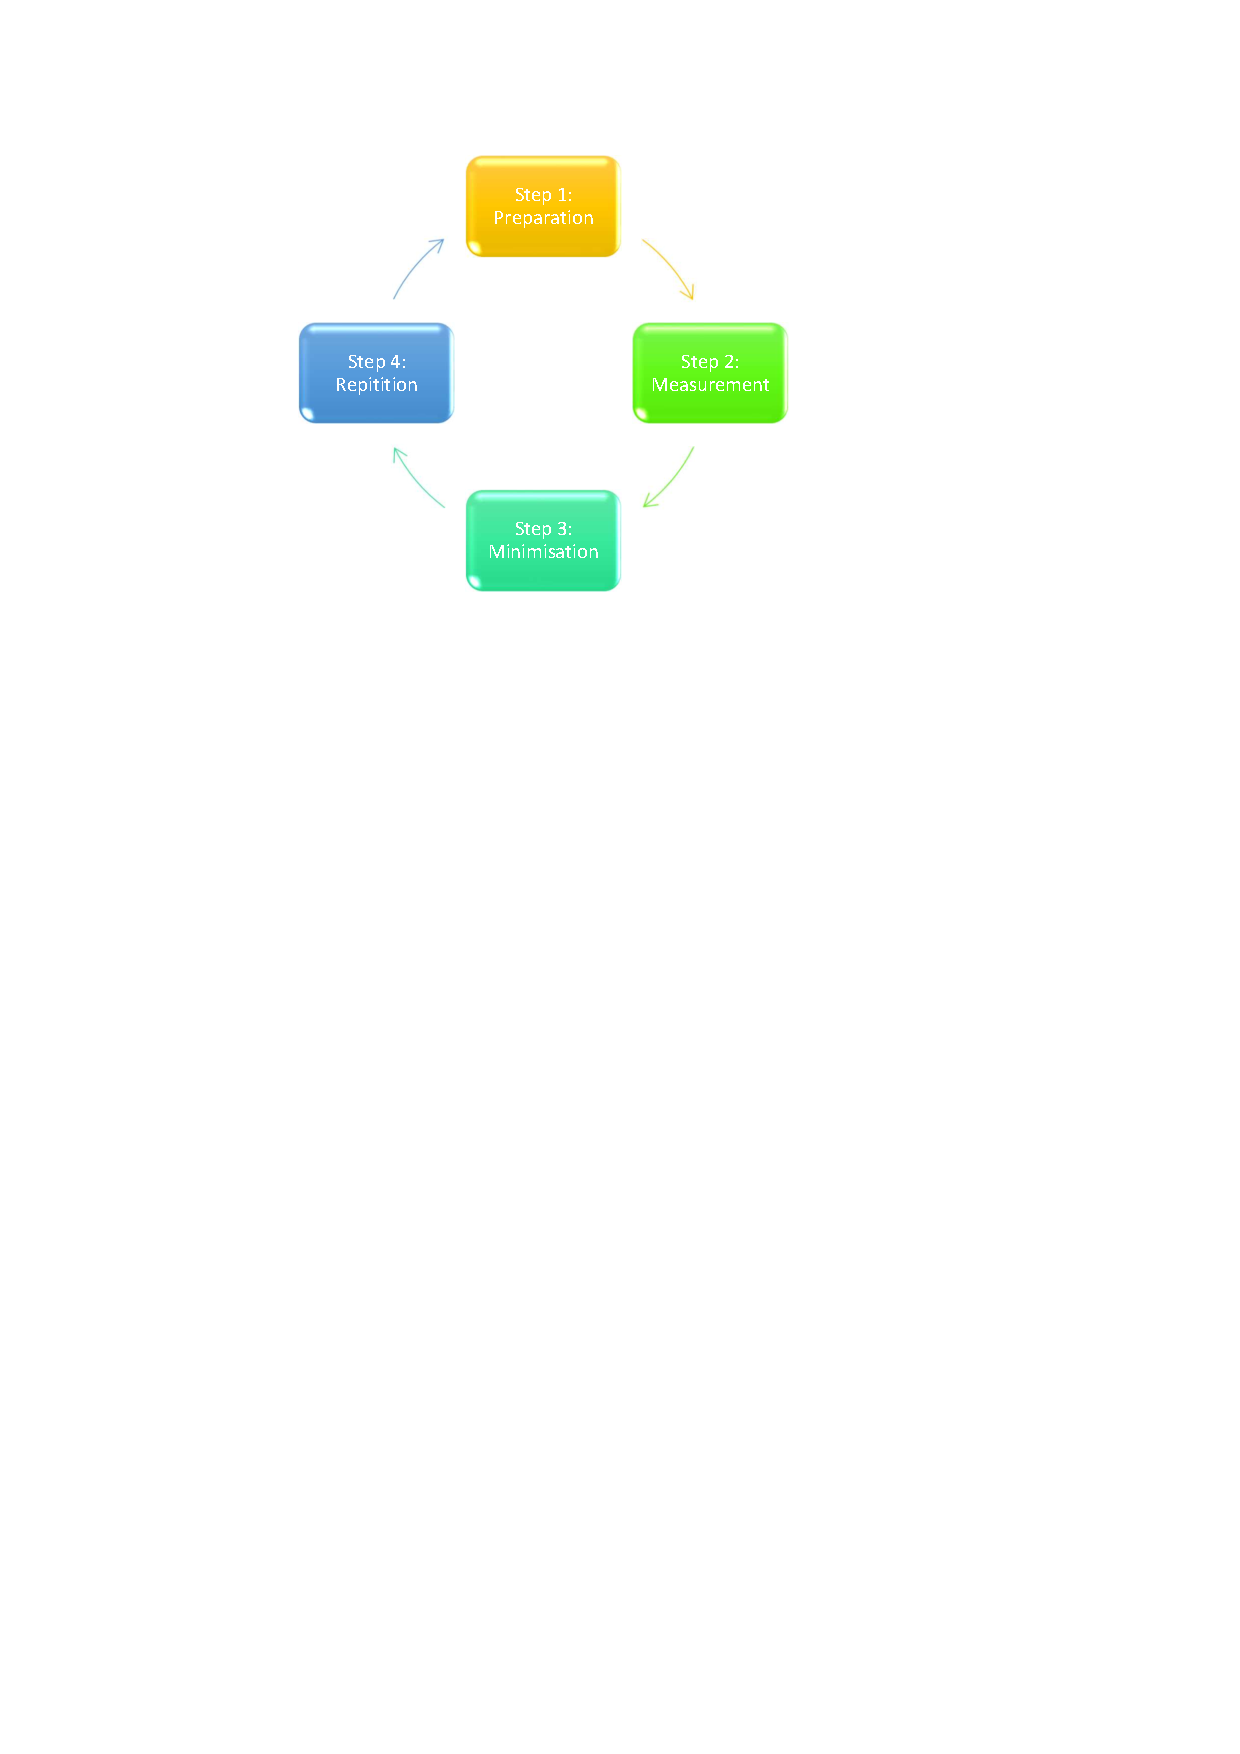
\includegraphics[scale=1]{VQEdiagram.pdf}
\end{center}
\caption{VQE flowchart}\label{VQE}
\end{figure}

\noindent
\setlength{\fboxsep}{0.5em}
\fbox{\begin{minipage}[c]{31em}%
 \centerline{\textbf{VQE}}
In 2014, the VQE algorithm was created by Alberto Peruzzo and Jarrod McClean. VQE comprises of classical and quantum features making it possible
 to use both classical and quantum resources to determine solutions to problems that are difficult to solve using a classical computer. The flow
 chart indicates the key instructions of implementing the VQE algorithm. The steps are explained in further detail as follows:

\begin{enumerate}
\item Preparation: Prepare the initial state of the system in terms of the variable theta by applying a quantum circuit. Implementing the unitary coupled cluster (UCC) method enables the algorithm to predict the ground state.
\item Measurement: Measure each local Hamiltonian, $H_{\gamma}$  and its corresponding scalar $g_{\gamma}$ to find the average value of the Hamiltonian \cite[p.2]{o2016scalable}.
\item Minimisation: Use a classical tool to find new solutions of theta in order to find the minimum eigenenergy of the Hamiltonian.
\item Repetition: By feeding the settings for $\vec{\theta}$ into the classical minimisation routine, the new settings for a new parameter of $\vec{\theta}$ i.e. $\vec{\theta}^{\prime}$. This process is repeated for n iterations until the parameter converges towards to specific value; this will enable an ideal state of the system to be obtained. From this, one can deduce a particular value for $E_{0}$, the smallest energy eigenvalue.
\end{enumerate}
 \end{minipage}}

\subsection{The Quantum Phase Estimation Algorithm (PEA)}
Similarly, to the VQE algorithm, one must ensure that the system is prepared in an initial state, but with the exception that the state must have a
 sufficient overlap with the ground state. Once the state is prepared in our desired state, an approximation is applied to the phase of the operator.
  The operator $\hat{U} = e^{-iHt}$ enables the initial state $\ket{\psi(0)}$ to change over time to the state $e^{-iEt}\ket{\psi(0)}$. Consequently,
  the initial state is mapped onto a superposition state of various qubits, which is called the ancilla qubits. After that, the state is acted on in
  turn inducing a phase on the system. Since the way in which the system evolves is controlled, it is now entangled with the initialised state.
 Next, we measure the phase obtained corresponding to each value of energy. The system as a result collapses to a single state with an associated
 probability. We repeat this algorithm for a higher number of ancilla qubits \cite[p.2]{tansuwannont2015quantum} until the lowest eigenenergy is
  obtained, or more precisely the energy of the ground state.

\begin{figure}[H]
\begin{center}
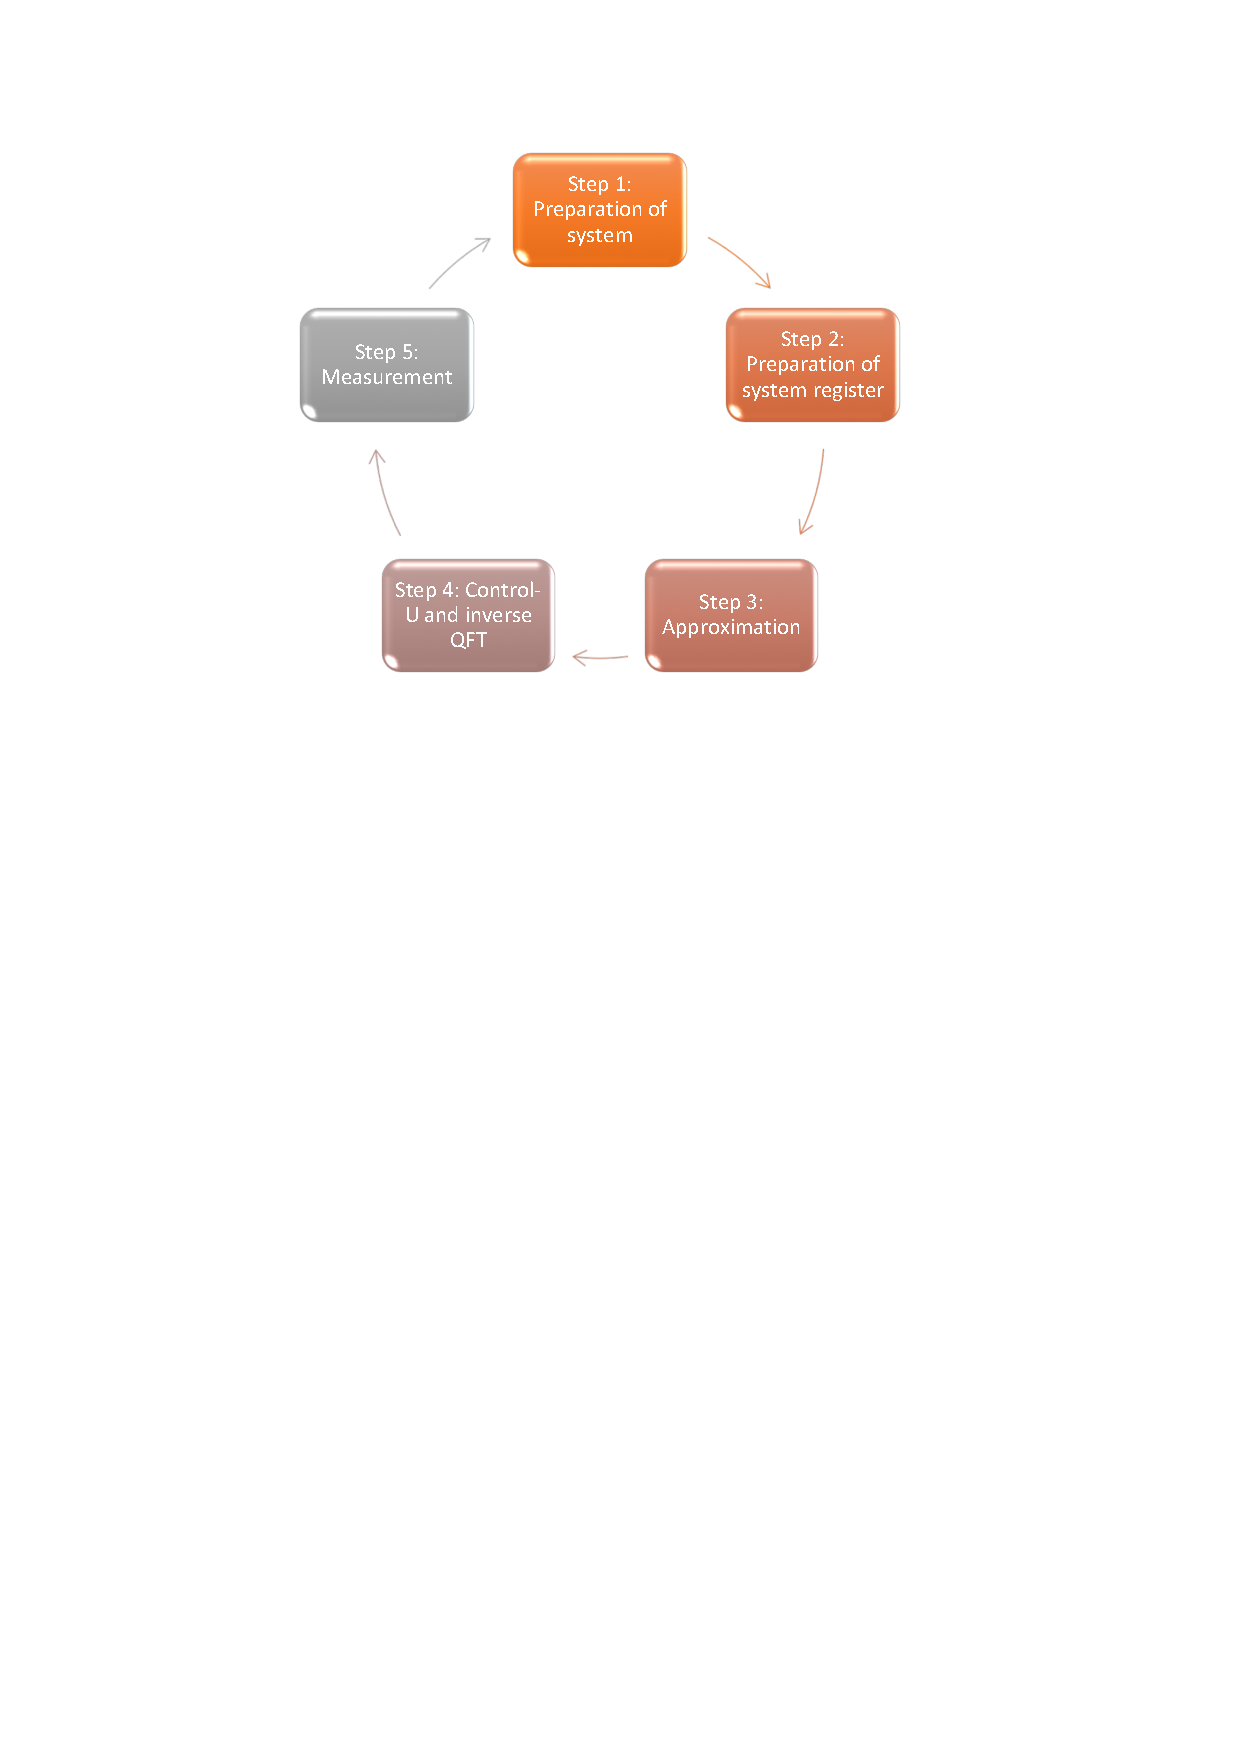
\includegraphics[scale=1.1]{PEA.pdf}
\end{center}
\caption{PEA flowchart}
\end{figure}

\noindent\setlength{\fboxsep}{0.5em}
\fbox{\begin{minipage}[c]{31em}%
\centerline{\textbf{PEA}}
The PEA is a quantum subroutine of the original quantum algorithm for chemistry used to computer eigenenergies of a given molecular structure. As any state $\ket{\psi(t)}$ evolved by unitary can be represent
 by applying phase difference onto initial state $e^{-iEt}\ket{\psi(0)}$. Phase estimation algorithm (PEA) is used then to find this relative phase and
  convert it into energy. In order to preform PEA we need to prepare two parts of qubits. First n qubits of superposition state
   $\frac{\ket{0} + \ket{1}}{\sqrt 2}$, second, our initial state. Since we can evolve states by unity operator. By inputting both parts of qubits
   onto a multiple controlled-U gate, the eigenvalue of each unitary $\hat{U}$ will transform to each one of qubits in first part.

Now let us recap Quantum Fourier Transformation, one transforms the tensor product of multiple states onto phase of some superposition states:
\begin{footnotesize}
\[
	\ket{j_{1} j_{2} \cdots j_{n}}\rightarrow \frac{\overbrace{\left(\ket{0}+e^{2 \pi i 0. j_{n}}\ket{1}\right)\left(\ket{0}+e^{2 \pi i 0. j_{n-1} j_{n}}\ket{1}\right) \cdots\left( \ket{0}+e^{2 \pi i 0. j_{1} j_{2} \cdots j_{n-1} j_{n} }\ket{1}\right)}^{\text{our prepared superposition qubits}}}{2^{\frac{n}{2}}}.
\]
\end{footnotesize}
As we can see, the result of QFT is just the first part of qubits we prepared. Therefore we would apply the reverse QFT onto those qubits, and outputs a single state contains all information about phase we want. The algorithm then deduces the relative phase and converts it into energy.
\end{minipage}}


\subsection{The Experimental Implementation}

The most widely accepted prerequisites to build a viable physical quantum computing technology were proposed by the American physicist
David DiVincenzo in 2000, with a few additional conditions added since. The original five DiVincenzo Criteria are:

\begin{enumerate}
\item Scalable physical system of well-characterised qubits.
\item Ability to initialize the state of the qubits to a simple fiducial state.
\item Long decoherence times, much longer than the “gate-operation” time.
\item Universal set of quantum gates.
\item Qubit-specific measurement capability.
\end{enumerate}

Now there are a number of different approaches to building physical quantum computing hardware being pursued by various research groups
and companies, each with their own pros and cons. Some of the types of implemented qubits include trapped ions, nitrogen-vacancy centres,
 quantum silicon photonics and superconducting, to name but a few. The type used here is the Xmon transmon qubit, a superconducting qubit
  built around a superconducting quantum interference device, or SQUID. Variations of the superconducting qubit are being developed by
  companies such as D-wave, IBM and Rigetti in the current race for quantum supremacy.

\noindent\setlength{\fboxsep}{0.5em}
\fbox{\begin{minipage}[c]{31em}%
\centerline{\textbf{Experimental realisation (SQUID)}}
The physical hardware used for implementing the VQE and PEA algorithms is an Xmon qubit which is a variation of the transmon qubit, a class of
superconducting interference device or SQUID. It is a type of charge qubit, which is to say it is a qubit where it’s ‘0’ and ‘1’ basis states are
charge states, and the superposition of these charge states is tuned using microwave resonators. The Xmon qubit has a number of favourable features,
 which include easy fabrication, fast qubit control and long qubit coherence times.

Using superconducting qubits is an appealing option for quantum hardware because it provides the scalability which is lacking for some other types
 of qubit. This is on account of the fact that for superconductivity the conduction electrons condense to a macroscopic quantum state which
 facilitates the creation of large integrated quantum circuits.

The Xmon qubits are placed inside a dilution refrigerator which is at a temperature of 20mK. The inter-qubit coupling, and qubit measurement
and control, are all done using microwave resonators. Single (or local) quantum gates are achieved using pulses of microwave radiation.
The entanglement operation used is the controlled-Z or CZ gate, this is achieved by fixing the frequency of one qubit while adiabatically
tuning the other qubit from the $\ket{11}$ state to near to the $\ket{02}$  state, which gives a relative phase shift. \end{minipage}}

\section{Main Achievement of paper}
As it is known, building a quantum computer comes with many challenges, one being the aspect of scalability. One of the advantages of using PEA to
compute electronic structures of a molecule is better asymptotic scaling which would prove useful for larger molecules than Hydrogen. However, this
is problematic as one would need to utilise more steps in the Trotterisation approximation which would in turn incur higher exponential costs. Hence,
 it was determined that a single Trotter step is not enough to accurately predict chemical rates for a Hydrogen molecule. In addition, for a single
 trotter step, each simulation using PEA was ran using different orderings of local Hamiltonians in order to find the optimal Trotter sequence for
 each bond length. For larger molecules, this is deemed intractable which becomes extremely difficult for the preprocessing requirements for a
 classical computer.

On the contrary, VQE was proved to be more effective due to its robustness to error. This is due to its success in predicting the chemical dissociation
 rate below the chemical accuracy threshold. Due to its short measurement sequences, it is more viable to use VQE for quantum simulations.
 Consequently, the quantum coherence of the system would be preserved which would limit the quantum error correction.

Although a quantum simulation such as the VQE is almost foolproof it may still not be adequate to calculate exact numerical solutions that are
characteristic of various types of molecules and their interactions. Quantum computing shows promise to eliminate such errors whilst using a
larger number of qubits. However, these factors work against each other. If such a machine can be built, there would be more states and thus
information to manipulate whilst withstanding error. This could revolutionise applications such as pharmaceuticals where cures and treatments
 for complex or incurable diseases such as Cancer, Prion disease and so forth could be engineered. If (or when should I say) this is possible,
  we would have a machine taking on the roles of a chemist, problem solver and designer simultaneously and combined into one entity!

\section{Conclusion and outlook}
As this is the first scalable simulation of molecular energies on any type of quantum hardware it represents an important step in the history of
quantum computing applications. The results indicate that for near-term quantum devices without effective error correction the adaptive approach
represented by the Variational Quantum Eigensolver may have better error resilience than that of standard gate model approach represented by the
Phase Estimation Algorithm. The expectation is that this work will pave the way for the development of further techniques for intractable calculations
 in quantum chemistry. And the final aim is that eventually these variational quantum chemistry techniques will allow for numerically exact simulations
  of chemical reaction rates, which are of great industrial commercial value. In particular, the efficiency - requiring only short state preparation
   and measurement procedures, and so it is without the normal substantial overhead required for quantum error correction - and robustness to
   error displayed by the experimental implementation of the variational quantum eigensolver technique indicates that this technique might succeed
    where classical techniques fail in solving traditionally intractable problems.

Late last year the US passed the new National Quantum Initiative Act pledging around \textdollar1.2 billion in funding for quantum information science
 \cite{usbill}. At a similar time the EU commission launched the €1 billion Quantum Technologies Flagship which will fund over 5000 of the top
 European researchers in quantum technologies over the next decade \cite{eubill}. In the UK, the EPSRC-backed Quantum Technology Hubs represent
 part of a £270 million investment to create national networks of quantum expertise \cite{ukbill}. With this extraordinary push of late across
 Europe and also in the US and China, aiming to fast-track quantum technologies out of university research groups and into industrial applications,
 the importance of this work in quantum chemistry simulations cannot be overstated. As aside from the much touted almost pop-science status of
 quantum encryption, the myriad opportunities afforded by more efficient scalable quantum chemistry simulations looms large in garnering serious
 investor interest. The ability to run quantum simulations of the behaviour of molecules and materials is hoped offer new avenues for increasing
 our understanding of chemistry and enable the development of new medicines and materials in silico.




\bibliography{ref}
\end{document}
